% $Id$

\documentclass[titlepage]{book}
\usepackage{amsmath}
\usepackage{amsthm}
\usepackage{helvet}
\usepackage{courier}
\usepackage{makeidx}
\usepackage{latex8}
\usepackage{times}
\usepackage[bottom]{footmisc}
\usepackage{graphicx}
\usepackage{url}
\usepackage{cite}
\usepackage{listings}
\usepackage[usenames, dvipsnames]{color}
\usepackage[toc,page]{appendix}
\usepackage{ifpdf}

\ifpdf
\usepackage[pdftex,colorlinks,backref,bookmarks]{hyperref}
\else
\usepackage[hypertex,colorlinks]{hyperref}
\fi

\setlength \headsep{.25in}

\graphicspath{{images/}}

\lstset {
  keywordstyle=\color{Blue}\textbf,
  commentstyle=\color{OliveGreen}\textit,
  escapeinside={(*@}{@*)},
  showstringspaces=false,
}

\title{The Component Workload Emulator (CoWorkEr) Utilization Test Suite (CUTS) User's Manual}

\author{James H. Hill}

\begin{document}

\maketitle

% $Id$

\begin{abstract}
Enterprise distributed systems (such as air traffic management systems, 
cloud computing centers, and shipboard computing environments) are steadily 
increasing in size (e.g., lines of source code and number of hosts in the 
target environment) and complexity (e.g., application scenarios). To address 
challenges associated with developing next-generation enterprise distributed 
systems, the level of abstraction for software development steadily increases
as well. Distributed system developers therefore focus more on the system's
``business-logic'' instead of wrestling with low-level implementation details, 
such as development and configuration, resource management, fault tolerance. 
Moreover, increase the level of abstraction for software development helps
promotes reuse of the system's ``business-logic'' across different application 
domains, which inherently reduces (re)invention of core intellectual property.

Although increasing the level of abstaction for software development is improving 
the software lifecycle of next-generation enterprise distributed systems, system 
quality-of-service (QoS) properties (\textit{e.g.}, latency, throughput, and 
scalability) are not evaluated until late in the software lifecycle, \textit{i.e.}, 
during system integration time. This is due in part to the \textit{serialized-phasing 
developmen problem} where the infrastructure- and application-level system entities, 
are developed during different phases of the software lifecycle. Consequently, 
distributed system developers do not realize the system under development does 
not meet its QoS requirements until its too late, \textit{i.e.}, during complete 
system integration time.

System execution modeling (SEM) tools is a model-driven engineering technique
that helps overcome the effects of serialized-phasing development. SEM tools
provide distributed system developers with the necessary artifacts and tools 
for modeling system behavior and workload, such as computational attributes, 
resource requirements, and network communication. The constructed models are
then used to evaluate QoS properties of the system under development during
early phases of the software lifecycle. This enables distributed system 
developers to pinpoint potential performance bottlenecks before they become
to costly to locate and rectify later in the software lifecycle.

The Component Workload Emulator (CoWorkEr) Utilization Test Suite (also known  
as CUTS) is a SEM tool designed for next-generation enterprise distributed 
systems. Distributed system developers and testers use CUTS to model the expected behavior 
and workload of the system components under development using high-level
domain-specific modeling languages. Model interpreters then transform the 
constructed behavior and workload models into source code for their target 
architecture, \textit{i.e.}, the components same interfaces and attributes as 
their real counterpart. Finally, system developers and testers emulate the 
auto-generated components in their target (or representative) environment
and collect QoS metrics. This enables distributed system developers and testers
to conduct system integration test at early stages of software lifecycle,
instead of waiting until complete system integration time to perform such
testing.

\iffalse
Developers and testers can grapically view the collected metrics while the system 
is executing to understand its current performance, and gain insight on how to 
improve it. Developer also have the option of viewing and analyzing collected 
performance metrics postmortem. Lastly, as the real component's implementation 
is completed, it can replace its respective emulation component to produce more 
realistic results and facilitate continuous system integration.
\fi

This book therefore is the end-user's guide to CUTS. It contains information on 
building and installing CUTS, using its domain-specific modeling languages to model
behavior and workload, creating system experiments, and details on CUTS many tools 
that help simpify evaluting QoS of next-generation distributed systems continuously
throughout the software lifecycle.
\end{abstract}


\tableofcontents

% $Id$

\part{Getting Started}

% $Id$

\chapter{Building and Installing CUTS}
\label{chap:install}

CUTS has many small projects that comprise the entire system execution modeling
(SEM) tool. Its many projects, however, can be divided into three main toolsets:
\begin{itemize}
  \item Runtime architecture
  \item Modeling tools
  \item Analysis tools
\end{itemize}
This chapter discusses how to build and install each of the aforementioned
toolsets for CUTS. Depending on your usage of CUTS, you may not need to build 
and install all projects in a category on the same machine. For example, you 
may install the runtime toolset of CUTS in your testing environment, and 
the modeling and analysis toolset outside of your testing environment to 
minimize interference with the testing process when viewing collected 
performance metrics in real-time. We are aware of these needs, and have 
setup the build process to decouple projects within a toolset from projects 
external to its corresponding toolset. You can, therefore, refer to each of the 
following sections on building and installation in isolation since toolsets do 
not explicitly depend on each other.

\section{CUTS Runtime Toolset}
\label{sec:install-runtime}

The runtime toolset for CUTS allows developers and testers to emulate system 
experiments on their target architecture. CUTS also provides the mechanisms
to monitor and collect performance metrics for the executing system. In order to 
build the CUTS runtime architecture, you will need the following technologies 
installed on the target machine(s):
\begin{figure}[htbp]
  \centering
  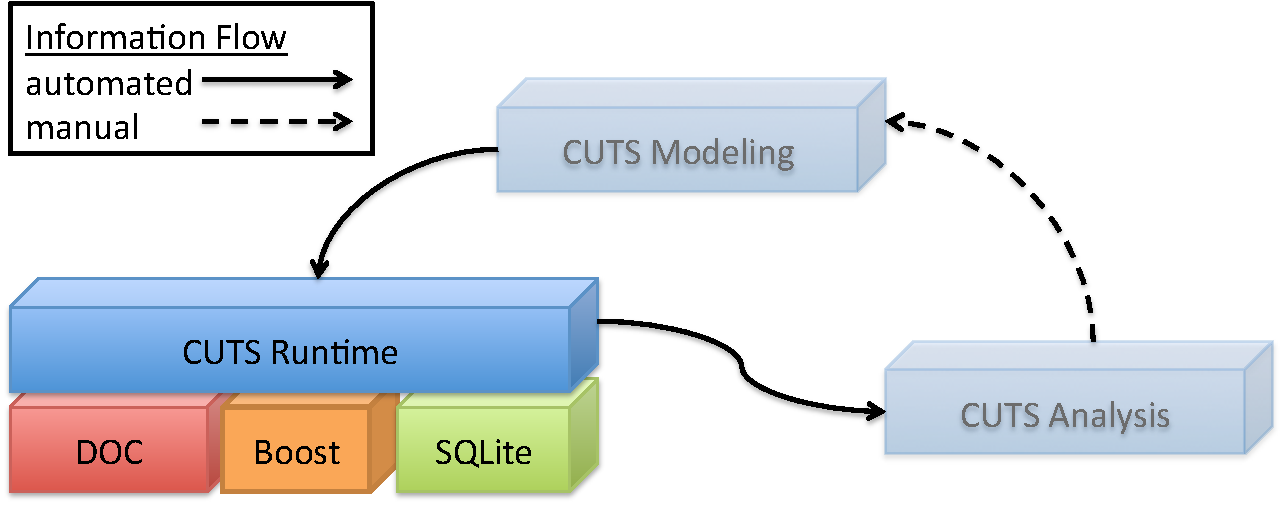
\includegraphics[scale=0.5]{cuts-runtime-blocks.pdf}
  \caption{Building blocks for the CUTS runtime architecture}
  \label{fig:cuts-runtime-blocks}
\end{figure}

\begin{itemize} 
  \item \textbf{DOC Group Middleware} - This set of middleware is used to abstract 
  away complexities associated with implementing applications that operate on many 
  different operating systems (ACE) and perform distributed communication (TAO). 
  You can download DOC Group Middleware from the following location: 
  \url{http://www.dre.vanderbilt.edu}.

  \item \textbf{Boost} - This set of libraries is used for implementing the parsers 
  (Boost Spirit) used within different artifacts of CUTS. You can download Boost from
  the following location: \url{http://www.boost.org}.

  \item \textbf{SQLite} - This set of libraries is used to support flat file archives
  for test results. You can download SQLite at the following location: 
  \url{http://www.sqlite.org}.

  \item \textbf{PCRE (not pictured)} - This set of libraries is used to enable PERL 
  regular expression support in CUTS. You can download PCRE at the following location:
  \url{http://www.pcre.org}.

  \item \textbf{XSC (not pictured)} - This set of libraries and applications is used to 
  convert XML documents to/from objects. You can download XSC from the following location: 
  \url{svn://svn.dre.vanderbilt.edu/XSC/trunk}.
\end{itemize}

\subsection{Obtaining Source Files}
\label{sec:install-download-runtime}

You can obtain the latest snapshot of the CUTS runtime architecture from the
DOC Group Subversion repository at the following location:
\begin{lstlisting}
(*@\url{svn://svn.dre.vanderbilt.edu/DOC/CUTS/trunk/CUTS}@*)
\end{lstlisting}
If you need to download a stable version of the source code, then you can 
access at one of the subdirectories in the repository at the following location:
\begin{lstlisting}
(*@\url{svn://svn.dre.vanderbilt.edu/DOC/CUTS/tags}@*)
\end{lstlisting}

\subsection{System Configuration}

Before you can build CUTS, you must for configure you environment. Please
set the following environment variables:
\begin{lstlisting}
%> export CUTS_ROOT=location of CUTS
%> export LD_LIBRARY_PATH=$LD_LIBRARY_PATH:$CUTS_ROOT/lib
%> export PATH=$PATH:$CUTS_ROOT/bin
\end{lstlisting}
Please see Appendix~\ref{chap:thirdparty} for instructions for configuring,
building, and installing third-party libraries needed by CUTS, such as 
DOC Group Middleware, Boost, and SQLite.

\subsection{Installation}

We use Makefile, Workspace, Project Creator (MPC)~\footnote{For more information
on MPC, please see the following location: \url{http://www.ociweb.com/products/mpc}}
to assist in building CUTS
on different operating systems, and with different compilers. Before you can
build the runtime architecture, you must first generate the target workspace.
Use the following command to generate the workspace:
\begin{lstlisting}
%> $ACE_ROOT/bin/mwc.pl -type TYPE [-features FEATURES] CUTS.mwc
\end{lstlisting}
where TYPE is your compiler type, and FEATURES is a comma-separated list of 
features
for your build of the CUTS runtime architecture.\footnote{You can type 
\texttt{\$ACE\_ROOT/bin/mwc.pl --help} to view the command-line options for 
MPC.} The complete set of features for CUTS is located in 
\texttt{\$CUTS\_ROOT/default.features.tmpl}. It is recommended that you copy 
the template feature file to \texttt{\$CUTS\_ROOT/default.features}
and set the appropriate features for your workspace by 
modifying the new file. This way you do not have to use 
the \texttt{-features} command-line option unless you want
to override your default feature selection. Once you have generated 
the workspace, you can build the solution using your specified compiler.

\section{CUTS Modeling Toolset (Windows-only)}

CUTS modeling tools provide system developers and testers with an enviroment
for rapidly constructing experiments for distributed component-based systems,
and generating testing system for their target architecture. The modeling
tools are built on the following technologies:
\begin{figure}[htbp]
  \centering
  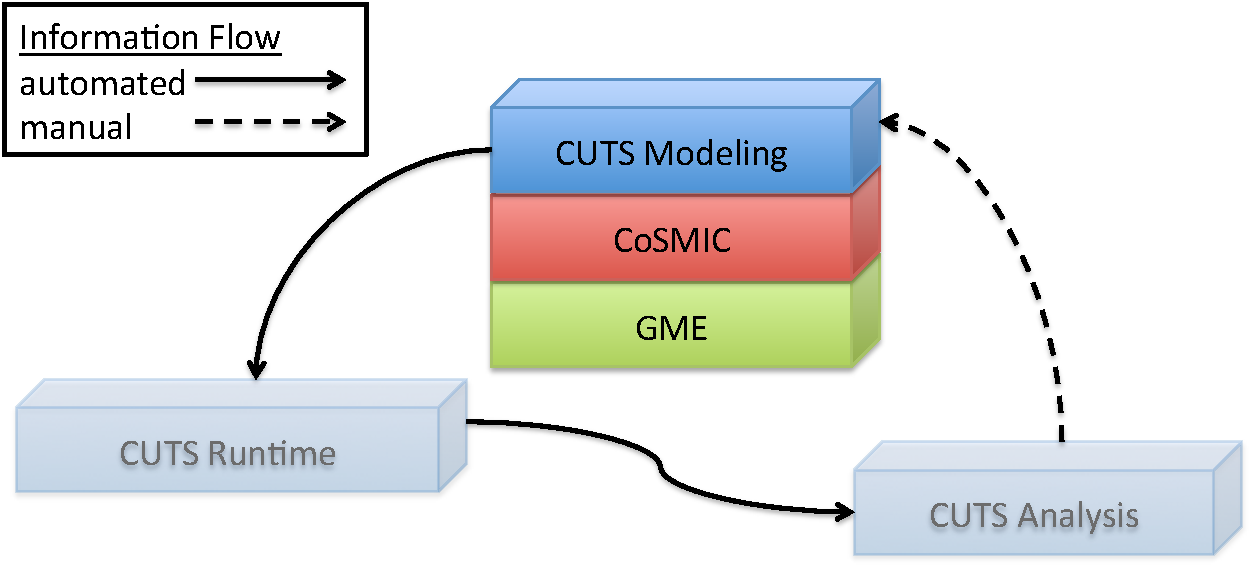
\includegraphics[scale=0.5]{cuts-modeling-blocks.pdf}
  \caption{Building blocks for the CUTS modeling tools}
  \label{fig:cuts-modeling-blocks}
\end{figure}

\begin{itemize}
  \item \textbf{GME} - The Generic Modeling Environment (GME) is a graphical
  modeling tool for creating domain-specific modeling languages (DSMLs). You
  can download GME from the following location: \url{http://www.isis.vanderbilt.edu/projects/GME}.

  \item \textbf{CoSMIC} - The Component Synthesis via Model Integrated 
  Computing (CoSMIC) is a tool suite designed to address the complexities of
  building large-scale component-based systesm, such as sytem assembly, 
  deployment, packaging, and planning. You can download CoSMIC from the following
  location: \url{http://www.dre.vanderbilt.edu/cosmic}.
\end{itemize}

\subsection{Installing Prebuilt Version}

The easiest and quickest way to install the CUTS modeling tools is to install
them using the .msi installer. You can download the latest version of the 
CUTS modeling tools from the following location:~\url{http://www.dre.vanderbilt.edu/CUTS/downloads}.
Before you can install the CUTS modeling tools, please make sure you have
installed GME and CoSMIC. Once both GME and CoSMIC are installed (in that
order), then you can install the CUTS modeling tools.

\subsection{Building from Sources (advanced)}

If you choose, you can build the modeling tools from source. This is given you
have downloaded all the source from the CUTS source code repository (see 
Section~\ref{sec:install-download-runtime}). To build the CUTS modeling tools,
first install the latest version of GME. Then, you \textbf{MUST} build CoSMIC
from source as well. This is required because the CUTS modeling tools are
built on top of CoSMIC, and its therefore dependent on CoSMIC. You can find
instructions for building CoSMIC from source at the following location:
\begin{lstlisting}
(*@\url{http://www.dre.vanderbilt.edu/cosmic/downloads}@*)
\end{lstlisting}
After you have built and installed CoSMIC from sources, you are ready to build
the CUTS modeling tools from source. Please use the following commands to 
build the modeling tools using your flavor of Visual C++:
\begin{lstlisting}
%> cd %CUTS_ROOT%
%> mwc.pl -type [vc type] -features modeling=1,cosmic=1 CUTS_CoSMIC.mwc
%> open solution and build
\end{lstlisting}
The build process will ensure that all the interpreters are installed
and configured for your environment.

\section{CUTS Analysis Toolset}

The CUTS analysis tools allow developers to view and analyze system
performance metrics. The analysis tools are developed using the following
key technologies:
\begin{figure}[htbp]
  \centering
  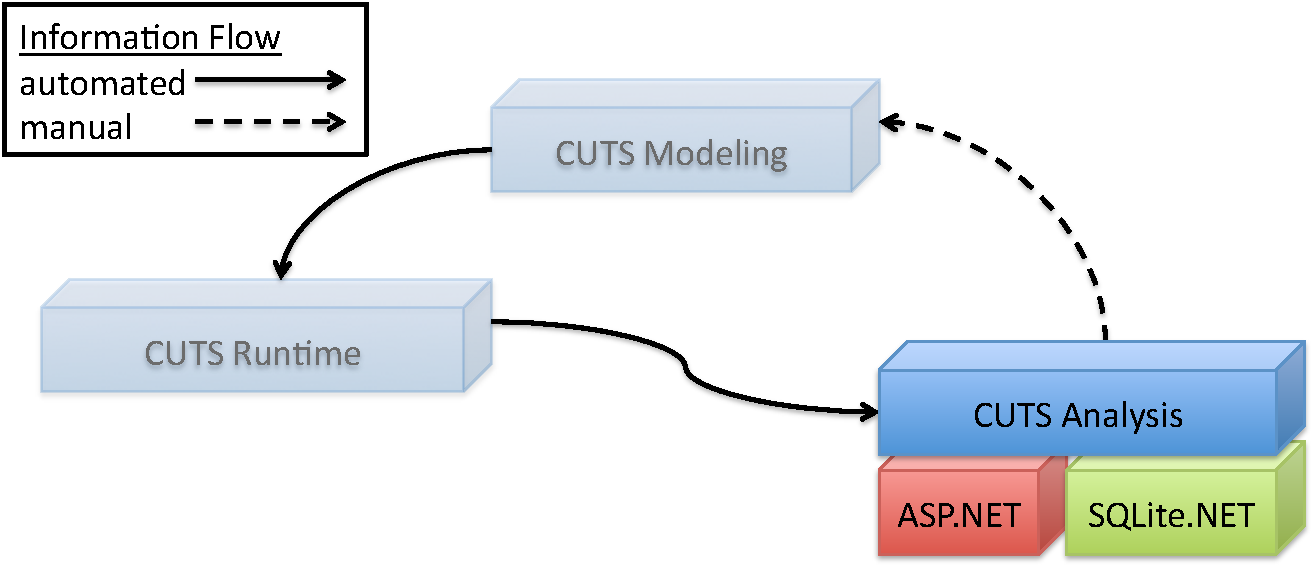
\includegraphics[scale=0.5]{cuts-analysis-blocks.pdf}
  \caption{Building blocks for the CUTS analysis tools}
  \label{fig:cuts-analysis-blocks}
\end{figure}

As shown in Figure~\ref{fig:cuts-analysis-blocks}, the same technologies 
used to develop the runtime toolset (see Figure~\ref{fig:cuts-runtime-blocks}) 
are used to develop the analysis toolset. Because the same technologies 
are used in the analysis toolset, the core projects in analysis toolset 
is also built while building the runtime toolset.
\iffalse
\begin{itemize}
  \item \textbf{ASP.NET} - ASP.NET is used to create the web application
  for the analysis tools, which is the main access portal for viewing 
  test results.

  \item \textbf{SQLite.NET} - SQLite.NET is the embedded database technology
  we use to manage the backend database(s). You can download SQLite.NET
  from the following location:~\url{http://sqlite.phxsoftware.com}
\end{itemize}

\subsection{Installing Prebuilt Version}

The easiest and quickest way to install the CUTS analysis tools is to install
them using the .msi installer. You can download the latest version of the
CUTS analysis tools from the following location:
\begin{lstlisting}
(*@~\url{http://www.dre.vanderbilt.edu/CUTS/downloads}@*)
\end{lstlisting}
Before you can install the CUTS modeling tools, please make sure you have
installed ASP.NET 2.0 and SQLite.NET. Once both ASP.NET 2.0 and SQLite.NET are 
installed, then you can install the CUTS modeling tools.~\footnote{We assume that 
Microsoft Internet Information Services (IIS) is already installed on the server
that you installing the CUTS analysis tools. Otherwise, please install Microsoft
IIS before installing the CUTS analysis tools, or any of its dependencies.}~\footnote{We
currently do not support Mono. Future versions of the CUTS analysis tools, however, will
support Mono.}

\subsection{Building from Sources (advanced)}

If you choose, you can build the CUTS analysis tools from source. This is given 
you have downloaded all the source from the CUTS source code repository (see
Section~\ref{sec:install-download-runtime}). To build the CUTS analysis tools,
first install Visual Studio.NET 2003 or better. Afterwards, please use the following 
commands to build the analysis tools:
\begin{lstlisting}
%> cd %CUTS_ROOT%\utils\BMW
%> mwc.pl -type [vc8 | vc9] BMW.mwc
%> open solution and build
\end{lstlisting}
The build process will ensure that all assemblies and the website build correctly. 
Once the build process is complete, you will to register the following location
with Microsoft IIS: \texttt{\%CUTS\_ROOT\%$\backslash$utils$\backslash$BMW$\backslash$website}.
This will allow you to view the website from your favorite web browser.
\fi

 
%% $Id$

\chapter{Quick Start Tutorial}

This chapter provides a quick start tutorial for using CUTS. After reading this
chapter, you will have a basic understanding of how to:
\begin{enumerate}
  \item model application behavior and workload;

  \item generate a test system model the constructed model;

  \item execute the system in your target environment;

  \item collect and analyze test results.
\end{enumerate}
In this tutorial, you will be measuring the end-to-end response time a simple
client/\-server application that communicates using asychronous events. This
tutorial assumes you have basic understanding of the Generic Modeling 
Environment (GME), CoSMIC/\-PICML, and the CORBA Component Model (CCM). More specifically,
this turorial will target the Component Integrated ACE ORB (CIAO) 
middleware\footnote{CIAO is an open-source implementation of the CCM, and is freely 
available for download at the following location: \url{www.dre.vanderbilt.edu/CIAO}.}.
Although this tutorial targets CIAO, the experience gained from
this tutorial can be applied to any architecture CUTS supports.

\section{Modeling Behavior and Workload}
\label{sec:quickstart-modeling}

Using GME, open the following file: 
\begin{lstlisting}
(*@\texttt{\$(CUTS\_ROOT)/examples/PICML/GettingStarted.xme}@*)
\end{lstlisting}
This model contains the structure of the client/\-server application, and 
is usually the starting point for using CUTS within PICML. 
Currently, application behavior and workload is modeled in the \texttt{Behavior}
aspect of a component's interface definition in PICML. The components in the model
located at:
\begin{lstlisting}
(*@\texttt{GettingStarted/InterfaceDefinitions/GettingStarted/GettingStarted}@*)
\end{lstlisting}
already contain model elements for its input/\-output ports. What remains is associating
the correct behavior and workload with these input/\-output ports for emulation
purposes. First, let's add behavior and workload to the client component by 
assuming the client component should periodically send an event to the server.
Please complete the following steps:
\begin{enumerate}
  \item Add a \texttt{PeriodicEvent} model element to the active model and 
  set its name to \texttt{periodicPing} and its \texttt{Hertz} attribute to 
  10 (\textit{i.e.}, 10 events/sec). 
  
  \item Insert an \texttt{InputAction} element, change its name to 
  \texttt{periodicPing}, and connect the \texttt{PeriodicEvent} to 
  the \texttt{InputAction}.

  \item Insert a \texttt{State} element, connect it with the \texttt{InputAction}.

  \item Insert an \texttt{OutputAction}, connect it with the \texttt{State}.

  \item Insert and connect another \texttt{State}. 

  \item Connect the final \texttt{State} with the originating \texttt{InputAction},
  \textit{i.e.}, \texttt{periodicPing}, to signify end of the behavior.
\end{enumerate}
Figure~\ref{fig:gettingstarted-client-behavior} illustrates the complete behavior 
model of the client in PICML, which is implemented in the previous steps.
\begin{figure}
  \centering
  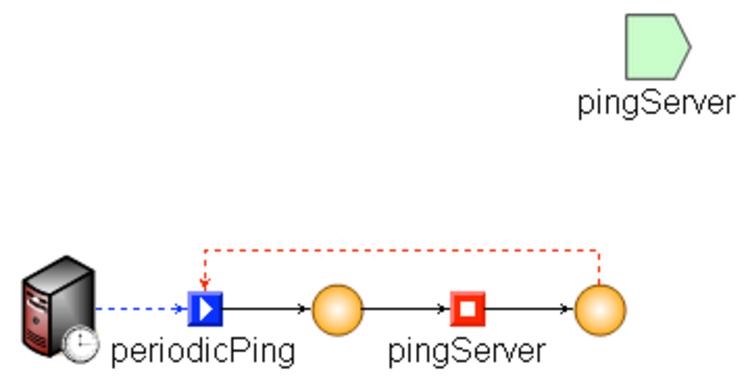
\includegraphics[scale=0.5]{gettingstarted-client-behavior.pdf}
  \caption{Client behavior model in PICML for CUTS emulation.}
  \label{fig:gettingstarted-client-behavior}
\end{figure}

\section{Generating Test System Implementation}
\label{sec:quickstart-generation}

After modeling the behavior and workload, the next step is to 
generate source code from the model. This will enable emulation 
of the test system on its target architecture. To generate source 
code from the model, launch the CUTS interpreter and excute the 
following steps (also illustrated in Figure~\ref{fig:quickstart-generate}):
\begin{enumerate}
  \item Select \texttt{Generate component implementation} radio button;
  \item Enter the target output directory;
  \item Select \texttt{Component Integrated ACE ORB (CIAO)} in the listbox;
  \item Click the \texttt{OK} button.
\end{enumerate}
Once the CUTS interpreter finishes generating source code, the IDL and CIDL 
files need to be generated in order to compile the source code. These files 
are created by the IDL Generator and CIDL Generator interpreters, respectively, 
provided with CoSMIC~\footnote{Please ensure to generate the IDL and CIDL 
files in the same directory as the source code previously generated 
from the model.}. Finally, there will be a \texttt{GettingStarted.mwc} 
file (its name may be different) located in the output directory selected 
for source code generation. This is a Makefile, Project and Workspace Creator 
(MPC) workspace file that contains all the necessary information to sucessfully 
compile the generated source code. Use \texttt{ettingStarted.mwc} to generate 
the appropriate workspace and then compile it.

\section{Executing in Target Environment}
\label{sec:quickstart-execution}

One design goal of CUTS is to (re)use the same infrastruture used in the 
target environment. The \texttt{GettingStarted.xme} example uses the Deployment 
And Configuration Engine (DAnCE), which is included with CIAO's standard 
distribution, to deploy the test system. To deploy the CUTS stock quoter 
example, use the following steps~\footnote{CUTS has a distributed testing
framework that simplifies many of the complexities associated with running
distributed system tests. We will cover the CUTS testing framework in later
chapters}:
\begin{enumerate}
  \item Generate the flat deployment plan descriptors from the 
  \texttt{GettingStarted}  model. You can find instructions on generating 
  the flat deployment plan in the original stock quoter tutorial included 
  with CoSMIC.
  
  \item Use DAnCE to deploy the GettingStarted.cdp. The original stock 
  quoter tutorial in CoSMIC has instructions on how to deploy a solution. 
  Be sure, however, to update the \texttt{nodemap.dat} file to the appropriate
  hosts and their location.
\end{enumerate}
When the CUTS version of the GettingStarted example is deployed, the test
manager will periodic collect log messages from each host/\-client, and 
insert them into a SQLite database for postprocessing.

\section{Analyzing Test Results}
\label{sec:quickstart-analysis}



% $Id$

\part{CUTS Analysis Toolset}
\label{part:analysis-toolset}

\chapter{UNITE}
\label{chap:unite}

This chapter discusses the main tool called \textit{Understanding 
Non-functional Intentions via Testing and Experimentation (UNITE)} in the CUTS 
analysis tool set. 

\section{Overview}
\label{sec:unite-overview}

UNITE is a method and a tool for analyzing system execution 
traces and validating QoS properties. Its primary purpose
is to support validation for distributed software systems,
but it can be used to analyze QoS properties of any software
system which generates a system execution trace. 
UNITE analyzes distributed system QoS properties such as 
end-to-end response time, service time and throughput using system 
execution traces. System execution trace is a collection of log messages.
These log messages are related to an execution of the system during a user 
decided time period. 

The system execution traces are collected 
using CUTS logging facilities as described in Chapter~\ref{chap:logging}.
CUTS uses SQLite (\url{http://www.sqlite.org}) 
to store the system execution trace. SQLite is a very lightweight 
database management system, which have a very flat file system. For example 
the generated system execution trace is contained in a single file and when 
the distributed system testers want to analyze the QoS properties they 
just need to show the location of this file to UNITE with a configuration 
file. 

This chapter first covers main concepts in UNITE in Section ~\ref{sec:unite-concepts}. 
Then it describes main configuration files of UNITE in  Section ~\ref{sec:unite-config}. 
Finally it shows how to use UNITE as a command line tool to analyze 
a given system execution trace in Section ~\ref{sec:unite-invoke}.

\subsection{Concepts in UNITE}
\label{sec:unite-concepts}

Table ~\ref{table:execution-trace} shows a sample system execution trace 
as stored in a database for offline QoS analysis. The most important 
data for UNITE is stored in the \textit{Message} column of the table. 
All the concepts describes below uses the log messages in the \textit{Message} 
column of the following table.

\begin{table}[h, captionpos=b]
  \caption{An example system execution trace }
  \label{table:execution-trace}
  \begin{tabular}{lcccl}
  \hline
  \textbf{ID} & \textbf{Time of Day} & \textbf{Hostname} & \textbf{Severity} & \textbf{Message} \\
  \hline
  10 & 2011-02-25 05:15:55 & sender.cs.iupui.edu & INFO & Config: sent event 5 at 120394455 \\
  11 & 2011-02-25 05:15:55 & sender.cs.iupui.edu & INFO & Planner: sent event 6 at 120394465 \\
  12 & 2011-02-25 05:15:55 & receiver.cs.iupui.edu & INFO & Planner: received event 5 at 120394476 \\
  13 & 2011-02-25 05:15:55 & sender.cs.iupui.edu & INFO & Config: sent event 7 at 120394480 \\
  14 & 2011-02-25 05:15:55 & receiver.cs.iupui.edu & INFO & Effector: received event 6 at 120394488 \\
  15 & 2011-02-25 05:15:55 & receiver.cs.iupui.edu & INFO & Planner: received event 7 at 120394502 \\
  \end{tabular}
\end{table}


Before start using UNITE following concepts need to be understood.

\begin{itemize}
  \item \textbf{Log Formats} - Each log message in the system execution 
  trace is constructed from a well defined format- called a \textit{log format}.
  \textit{Log Formats} are high-level constructs that capture both constant 
  and variable portions of individual, but similar log messages in a system 
  execution trace. For example Listing~\ref{listing:log-format}  shows 
  two different log formats which capture the log messages in 
  the above system execution trace.
  
  \begin{lstlisting}[label=listing:log-format, caption=Log formats for QoS analysis.,
   captionpos=b]
   LF1: {STRING cmp_id}:sent event {INT event_id} at {INT sent}
   LF2: {STRING cmp_id}:received event {INT event_id} at {INT recv}
  \end{lstlisting}
  
  The variable portions of the log format is specified inside place holders ({}).
  The information captured in the variable portions of a log format represent 
  metrics that  are very useful in QoS analysis. In the above example the 
  distribution of the values for the variable \textit{event\_id}, with the time 
  variables \textit{sent, recv } can be used to determine the latencies of 
  different events. The variable portion of a log format consists of a variable 
  type and a variable name. Table~\ref{table:data-types} shows the data types 
  supported by UNITE.
  
 \begin{table}[h, captionpos=b]
  \centering
  \caption{UNITE data types}
  \label{table:data-types}
  \begin{tabular}{lccl}
  \hline
  \textbf{Type} & \textbf{Description} \\
  \hline
  INT & Integer data type \\
  LONG & Long data type \\
  STRING & String data type (There cannot be spaces) \\
  FLOAT & Floating-point data type \\
  \hline
  \end{tabular}
\end{table}
  
  \item \textbf{Log Format Relations} - The other main concept in UNITE 
  is Log Format Relations. Log Format Relations define a cause-effect 
  relationship among two log formats. For example in the above example
  \texttt{LF1} represents a sent event in the distributed system. And \texttt{LF2} 
  represents a receive event in the system. The sent event always 
  happens before the receive event. There for the log message corresponds 
  to a particular sent event occurs before the corresponding receive event.
  We say \texttt{LF1} is the cause log format and \texttt{LF2} is the effect log format. In 
  order to relate the two log messages distributed system testators can use 
  the \textit{event\_id} variable as follows.
  
  \texttt{LF1.event\_id = LF2.event\_id}
  
  \item \textbf{QoS analysis expressions} - After specifying Log formats and 
  Log format relations distributed system testers have to specify a QoS analysis 
  equation to get the results. For example in the above example in order to 
  get the average response time following equation can be used.
  
  \texttt{AVG(LF2.recv - LF1.sent)}
  
\end{itemize}

The next section ~\ref{sec:unite-config} shows how to specify above 
mentioned details using the configuration files in UNITE.

\section{Configuring UNITE}
\label{sec:unite-config}

UNITE uses two xml configuration files called, \textit{datagraph file} and 
\textit{unite file} for the configurations. The \textit{datagraph file} is used to 
specify the details of log formats and relations. The \textit{unite file} 
contains a reference to the \textit{datagraph file} and is used for the 
QoS analysis.

Listing~\ref{listing:example.datagraph} shows a sample \textit{datagraph file}. 

\lstinputlisting[label=listing:example.datagraph,
  caption=An example configuration file for UNITE datagraph.,
  captionpos=b,numbers=left]{analysis/example.datagraph}

\subsection{Datagraph Schema Definition}
\label{sec:datagraph}

This section discusses the details of the UNITE datagraph configuration 
based on its underlying XML Schema Definition.

\xmltag{<cuts:datagraph>}
This is the main tag for the datagraph configuration document. Its 
XML namespace must have the \url{http://cuts.cs.iupui.edu} definition. If it does
not have this definition, then UNITE will not execute further.

\xmltag{<name>}

This tag contains the name of the datagraph. This tag does not have 
any child tags.

\xmltag{<adapter>}

This tag contains the location of an external adapter module required for 
for UNITE to correctly analyze the QoS properties. This tag is not 
mandatory. It only needs when the system execution trace does not 
contain required properties for the QoS analysis. See section () SETAF 
for more details.

\xmltag{<logformats>}

This tag is a container for set of log formats that will be used in QoS 
analysis process. It may contain any number of logformat elements. 
Log formats can be specified in any order .In general, cause log format 
is specified first. Then its effect log format is specified. 
The following is a list of child tags: \texttt{<logformat>}.

\xmltag{<logformat>}

This tag contains all the details about a particular log format. It has the following 
attributes.
\begin{table}[h]
  \begin{tabular}{lcccl}
  \hline
  \textbf{Name} & \textbf{Type} & \textbf{Default Value} & \textbf{Required} & \textbf{Description} \\
  \hline
  id & String  & & Yes & Name of the log format \\
  \end{tabular}
\end{table}

\noindent The following is a list of child tags:
\texttt{<value>}, \texttt{<relations>}.

\xmltag{<value>}
This tag contains the actual value of the log format. Value of a log 
format represent set of log messages in the system execution trace 
which have constant and variable parts as described in section (ref) 
This tag does not have any child tags.

\xmltag{<relations>}

This tag contains set of relations, in which the parent log format is 
involved in as the cause log format.
The following is a list of child tags: \texttt{<relation>}.

\xmltag{<relation>}

This tag contains all the details about a particular relation. Such 
as the effect log format and cause-effect variables. There can be 
more than one cause-effect variable pairs. It has the following 
attributes.
\begin{table}[h]
  \begin{tabular}{lcccl}
  \hline
  \textbf{Name} & \textbf{Type} & \textbf{Default Value} & \textbf{Required} & \textbf{Description} \\
  \hline
  effectref & String  & & Yes & The id of the effect log format in this relation \\
  \end{tabular}
\end{table}

\noindent The following is a list of child tags:
\texttt{<causality>}.

\xmltag{<causality>}

This tag represent the relationship between a variable in the 
cause log format and a variable in the effect log format. It has 
the following attributes.
\begin{table}[h]
  \begin{tabular}{lcccl}
  \hline
  \textbf{Name} & \textbf{Type} & \textbf{Default Value} & \textbf{Required} & \textbf{Description} \\
  \hline
  cause & String  & & Yes & The name of the cause variable \\
  effect  & String  & & Yes &  The name of the effect variable \\   
  \end{tabular}
\end{table}

Therefore the elements mentioned above represent the datagraph 
for a partiucar system execution trace. Depending on the QoS 
properties being analyzed a particular system execution trace 
may have more than one datagraphs. These different datagraphs 
may have different log formats and cause-effect relations.

In general the location of the \textit{datagraph file} is specified in the 
\textit{unite file}. Listing~\ref{listing:example.unite} shows a sample 
\textit{unite file}. 

\lstinputlisting[label=listing:example.unite,
  caption=An example configuration file for UNITE.,
  captionpos=b,numbers=left]{analysis/example.unite}

\subsection{Unite Schema Definition}
\label{sec:unite-scema}

This section discusses the details of the UNITE configuration 
based on its underlying XML Schema Definition.

\xmltag{<cuts:test>}
This is the main tag for the unite configuration document. Its 
XML namespace must have the \url{http://cuts.cs.iupui.edu} definition. If it does
not have this definition, then UNITE will not execute further.

\xmltag{<name>}

This tag contains the name of the unite file. This tag does not have 
any child tags.

\xmltag{<datagraph>}

This tag specify the location of the associated datagraph for the 
QoS analysis. This tag has the following attributes.

\begin{table}[h]
  \begin{tabular}{lcccl}
  \hline
  \textbf{Name} & \textbf{Type} & \textbf{Default Value} & \textbf{Required} & \textbf{Description} \\
  \hline
  location & String  & & Yes & The location of the datagraph configuration file. \\
  \end{tabular}
\end{table}

This tag does not have any child tags.

\xmltag{<evaluation>}

This tag contains the equation for QoS evaluation. The text inside 
this tag should be written in a certain way. The variables of this 
equation should be specified with the log format it belongs to. The 
dot operator after the log format specified the actual variable. This tag 
does not have any child tags.

\xmltag{<aggregation>}

This tag specifies a function used to convert a dataset to a single 
value. Some examples of aggregation functions are AVERAGE, 
MIN, MAX and SUM. This tag does not have any child tags.

\xmltag{<grouping>}

For a given aggregation function this tag tell how to classify 
datasets that are independent of each other. This is the 
container tag for such grouping items
The following is a list of child tags: \texttt{<groupitem>}. 

\xmltag{<groupitem>}

This tag represent an actual grouping item. The \textit{name} 
attribute specify the grouping item. This attribute consists of 
a particular log format id and a variable name. Their should be a 
\_ between the log format and the variable. This tag has the 
following attributes. 
\begin{table}
 \begin{tabular}{lcccl}
  \hline
  \textbf{Name} & \textbf{Type} & \textbf{Default Value} & \textbf{Required} & \textbf{Description} \\
  \hline
  name & String  & & Yes & The name of the grouping item. \\
  \end{tabular}
\end{table}

\xmltag{<services>}

UNITE has a facility to show the results of QoS analysis using different 
presentation methods such as graphs. There are many different presentation 
softwares available such as Microsoft Excel, Gnuplot. This tag contains the 
set of such services the testers want present the analyzed results. This tag has 
the following child tags:\texttt{<service>}

\xmltag{<service>}

This tag represent a presentation service. In general these presentation services 
are developed externally to UNITE and plugged in via a common interface.
Therefore child tags of this tag gives the details required to load these services 
during the runtime. This tag has the following attributes.

\begin{table}
 \begin{tabular}{lcccl}
  \hline
  \textbf{Name} & \textbf{Type} & \textbf{Default Value} & \textbf{Required} & \textbf{Description} \\
  \hline
  name & String  & & Yes & The name of the grouping item. \\
  \end{tabular}
\end{table}

\noindent The following is a list of child tags:
\texttt{<location>}, \texttt{<classname>}, \texttt{<params>}.

\xmltag{<location>}

This tag specify the location of a presentation service module. UNITE 
will search for this location when it wants to load the presentation 
service. This tag does not have any child tags.

\xmltag{<classname>}

This tag specify the name of the class of the presentation 
service. This tag does not have any child tags.

\xmltag{<params>}

This tag specify the additional parameters required to invoke 
the presentation service. This tag does not have any child tags.

\section{Invoking UNITE}
\label{sec:unite-invoke}

Assuming the CUTS runtime architecture has been built and installed 
correctly, the CUTS UNITE tool is installed at the following 
location:
\begin{lstlisting}
%> $CUTS_ROOT/bin/cuts-unite
\end{lstlisting}
To see a complete list of command-line options, use the following 
command:
\begin{lstlisting}
%> $CUTS_ROOT/bin/cuts-unite --help
\end{lstlisting}

A typical invocation of UNITE tool requires the data file which 
contains the system execution trace and the UNITE configuration 
file discussed above as arguments. The datagraph file location 
is specified inside the UNITE configuration file so it doesn't 
need to be specified as an argument. 
Assuming the configuration discussed above is defined in a file 
named \textit{example.unite},  and the system execution trace is resides 
in a file called \textit{example.cdb} you can run the CUTS UNITE tool with
the configuration via the following command: 
\begin{lstlisting}
%> $CUTS_ROOT/bin/cuts-unite -f example.cdb -c example.unite
\end{lstlisting}

% $Id$

\chapter{System Execution Trace Adaptation Framework (SETAF)}
\label{chap:setaf}

This chapter discusses a tool and a method called \textit{System 
Execution Trace Adaptation Framework (SETAF)} in the CUTS  analysis 
tool set. This tool is used as an extension to UNITE when analyzing QoS 
properties from system execution traces.

\section{Overview}
\label{sec:setaf-overview}

Chapter~\ref{chap:unite} discussed the method of UNITE when doing the 
QoS analysis using system execution traces. In some situations UNITE cannot 
be used alone to analyze system execution traces. This is because UNITE 
assumes that every different instance of a log format is unique. Which means 
it assumes that at least one log format variable other than the variable represent 
time have different values among different instances. This causes non-unique 
relations among different instances of log formats.

\begin{lstlisting}[label=listing:trace2, 
caption=Portion of a system execution trace that does not 
contain unique relations ., captionpos=b]
      Started doing task A at 12.00
      Finished doing task A at 12.01
      Started doing task A at 12.02
      Finished doing task A at 12.03
\end{lstlisting}

For example, Listing~\ref{listing:trace2} illustrates 
an example system execution trace where the dataflow graph
will not have unique relations between the log format. This 
is because it is \textit{hard} to know start/finish messages 
are associated with one another without human intervention.
Moreover, when an example similar to the one present in 
Listing~\ref{listing:trace2} is analyzed by UNITE, it 
will yield incorrect results because it is \textit{hard} to 
determine correct causality between similar log messages.

With proper planning early in the software lifecycle, it is
possible to ensure generated system execution traces have unique
relations to facilitate proper analysis. This, however, is not
alway possible---especially when analyzing system execution traces
generated by third-party systems and their components. Although
such system execution traces may not contain unique 
relations, the existing relations can be exploited (or adapted) 
to enforce a unique relation. For example, in 
Listing~\ref{listing:trace2}, although the relation is 
not unique, it can be adapted to be a unique relation by adding 
an id to each log message. This will ensure that UNITE analyzes 
the dataflow model and evaluates the expression correctly. 

Adding this kind of new ids means we have to add new log format 
variables to the identified log formats. Further new log format relations 
need to be identified for these newly added variables. Even though 
the ordinary log format variables get values from the system execution trace, 
it does not contain the values for these externally added log format 
variables.  Further the variables need to be added, the relations need 
to be enforced and what sort of values they get depend on the system 
execution trace being analyzed. Therefore UNITE provides a common 
interface for these task, but the implementation module should take 
care of how to adapt the dataflow model. Distributed system testers 
need to find out the adaptation patterns and need to provide these 
external adapters. 

Distributed system testers do not need to develop 
these modules using a language like C++. 
Instead SETAF provides a simple language 
to specify them as a adaptation specification. SETAF has a code 
generation tool to generate the source code for these adapters. After 
compiling these adapter modules, they need to be specified in the 
datagraph file so that UNITE can load them during the run time. The 
Figure~\ref{fig:setaf} showcase the overall workflow of SETAF.

\begin{figure}[htbp]
  \centering
  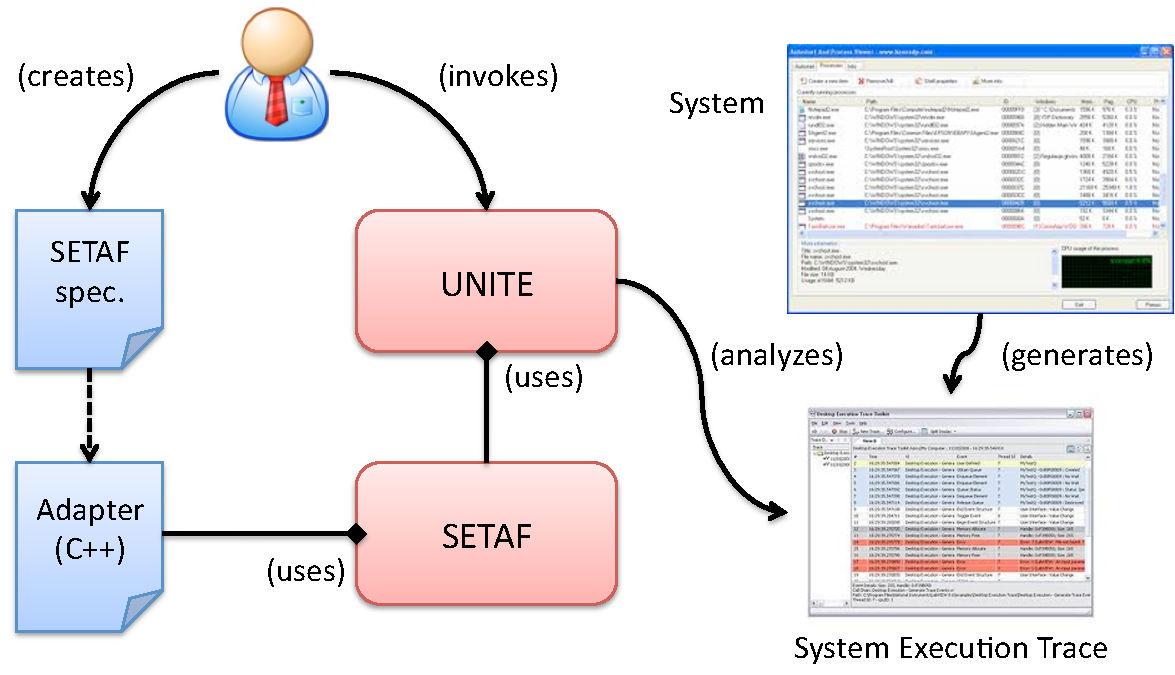
\includegraphics[scale=0.7]{analysis/setaf.pdf}
  \caption{Conceptual overview of SETAF's workflow.}
  \label{fig:setaf}
\end{figure}

The rest of the chapter describes the content of the UNITE Adapter 
Specification in Section~\ref{sec:unite-uas}. In Section~\ref{sec:code-gen} 
it describes the procedure of code generation of adapter modules in SETAF.
Finally Section~\ref{sec:qos-analysis} shows how to use SETAF with 
UNITE to do the QoS analysis. 

\section{UNITE Apater Specification}
\label{sec:unite-uas}

This section explains the content of Unite Adapter Specification. Listing
~\ref{listing:example.uas} shows an example of UNITE Adapter specification. 

\lstinputlisting[label=listing:example.uas,
  caption=An example UNITE Adapter Specification.,
  captionpos=b,numbers=left]{analysis/example.uas}


As shown in the listing the UNITE Adapter Specification has five sections (
\texttt{Variables, Init, Reset, Datapoints, Relations, Adaption code}). Following 
describes what data need to be specified in these different sections.
Please refer to the example provided above when reading the section 
below.

\begin{itemize}
  \item \textbf{Variables} - The adaptation module keeps the state
  of the adaption using the variables specified in this section. These 
  variables will be converted to private variables in the generated 
  C++ code. Let's call them state variables. 
  These state variables are used to populate values for 
  the newly added log format variables based on the state.

\item \textbf{Init} - The initial state of the adapter is specified in this 
  section. The declared variables in the above \textit{Variables} section 
  are initialized in this section.

\item \textbf{Reset} - Sometimes the variables representing the adapter state 
  may need to be reset. For example same state variable may be used 
  to populate values for different log format variables. In this case sometimes 
  the state variables need to reset when switching from one log format 
  to the other. This section is used for that.

\item \textbf{DataPoints} - This section specifies the log format variables 
  need to be added for the adaption. Each entry has a type and an identifier.
  The identifier has two parts, which are separated by a "." . Left side of the 
  separator contains the log format id and the right side contains the name 
  of the newly added log format variable. For an example \texttt{LF1.uid} means 
  a new variable named \texttt{uid} is added to the \texttt{LF1} log format.
  The type part specified the type of the log format variable. These log format variables 
  can have following types.

\begin{table}[h, captionpos=b]
  \centering
  \caption{UNITE data types}
  \label{table:setaf-data-types}
  \begin{tabular}{lccl}
  \hline
  \textbf{Type} & \textbf{Description} \\
  \hline
  INT & Integer data type \\
  LONG & Long data type \\
  STRING & String data type \\
  FLOAT & Floating-point data type \\
  \hline
  \end{tabular}
 \end{table}

\item \textbf{Relations} - This section specifies the relations which need be enforced 
  related to the the log format variables added in the \texttt{DataPoints} section.
  Each relation entry has two parts which are separated from a $\rightarrow$. 
  The left side of the $\rightarrow$ specifies the cause log format variable. And 
  the right side of $\rightarrow$ specifies the effect log format variable.

\item \textbf{Adaption code} - The adaption code is where the
  domain-specific logic resides for the adaption pattern. The
  adaption code is segmented based on the log formats that must
  undergo adaption. Each segment dictates how to update variables
  in the dataflow graph, as well as its own private variables. For 
  string variables the name of the variable and the value of the variable 
  are sufficient. For other types of variables a dynamic cast need to be 
  done as specified in the above example. 

\end{itemize}

\section{SETAF code generation}
\label{sec:code-gen}

The above descrIbed UNITE adapter specification will resides in a file 
which has \textit{.uas} extension. SETAF has a tool called \textit{cuts-setaf} 
to generate the adaptation source code using the adapter specification 
described above. Assuming the CUTS runtime architecture has been built 
and installed correctly, the CUTS SETAF tool is installed at the following 
location:
\begin{lstlisting}
%> $CUTS_ROOT/bin/cuts-setaf
\end{lstlisting}
To see a complete list of command-line options, use the following 
command:
\begin{lstlisting}
%> $CUTS_ROOT/bin/cuts-setaf --help
\end{lstlisting} 

For the code generation process two arguments need to be provided. The 
location of the UNITE adapter specification file and the directory 
location, to output the generated source code. As an example following 
invocation will generate the source code using the \textit{example.uas} 
file and the generated code will be output to the current directory.
\begin{lstlisting}
%> $CUTS_ROOT/bin/cuts-setaf -f example.uas -o .
\end{lstlisting}

This execution will output four files - \textit{source file, header file, 
project file and workspace file}. As an example the above invocation 
will generate \textit{example.h, example.cpp, example.mpc and example.mwc} 
files. Depending on the user preferred compiler the workspace for compiling 
the code can be created using Makefile, Project, and Workspace Creator (MPC).
As an example following shows how to create workspace for gcc and Visual 
Studio 2008 compilers.
For gcc:
\begin{lstlisting}
%> mwc.pl -type gnuace example.mwc
\end{lstlisting}

For Visual Studio 2008:
\begin{lstlisting}
%> mwc.pl -type vc9 example.mwc
\end{lstlisting}

In Linux like systems this will generate a dynamic link library with \textit{.so} extension.
Therefore in this case it will be example.so. In windows like systems this will create 
a dynamic link library with \textit{.dll} extension. Therefore in this case it 
will be example.dll.  

\section{QoS analysis with UNITE}
\label{sec:qos-analysis}

Section~\ref{sec:qos-analysis} described the process of generating the 
adapter module (the dynamic link library). The location and the name 
of this library is specified in the \texttt{<adapter>} tag of the datagraph 
file. See Section~\ref{sec:unite-config} for further details of datagraph 
file. UNITE will then load the adapter module from this location and 
use its functionality when required.

\chapter{(DMAC)}
\label{chap:dmac}


% $Id$

\appendix
\part{Appendix}

% $Id$

\chapter{Building and Installing Third-Party Libraries}
\label{chap:thirdparty}

The following appendix contains best practices for building
and installing third-party libraries used by CUTS projects. It is not
a requirement to install third-party libraries per the instructions in
this appendix. If you are experiencing compilation problems with CUTS
due to third-party libraries, however, the instructions in this appendix
may be of assistance. To make help explain the installation process
of the thirdparty libraries, it will be assumed that all third-party
libraries will be installed at the following location:
\texttt{/opt/thirdparty}\footnote{This location is representative 
of a common location for installing third-party libraries, and may
be different on your system.} \footnote{If you are installing CUTS
from source on Windows, it is recommended that you place all environment
variables in a BATCH file (\texttt{.bat}) so you do not pollute the
system environment.}.

\section{Boost}
\label{sec:thirdparty-boost}

The Boost libraries are required when building and installing CUTS. All
artifacts for Boost, such as prebuilt versions and source files, can be 
downloaded from the following location: \url{http://www.boost.org}. 

\subsection{System Configuration}

To build CUTS correctly, the Boost environment variables must be defined. Please 
define the following required environment variables:
\begin{lstlisting}
(*@\texttt{\%> export BOOST\_ROOT=} location of Boost@*)
(*@\texttt{\%> export BOOST\_VERSION=} name of subdirectery under \texttt{\$BOOST\_ROOT/include}, \textit{e.g.}, \texttt{boost-1\_34\_1}@*)
(*@\texttt{\%> export LD\_LIBRARY\_PATH=\$LD\_LIBRARY\_PATH:\$BOOST\_ROOT/lib}\footnote{On
Windows-based systems, please add library paths to \texttt{PATH}. On Mac OS-based
systems, please add library paths to \texttt{DYLD\_LIBRARY\_PATH}.}@*)
(*@\texttt{\%> export PATH=\$PATH:\$BOOST\_ROOT/lib}@*)
\end{lstlisting}
In some cases, Boost libraries will have an optional configuration appended to 
their filename, such as \texttt{-mt-d}. To use a specific configuration of 
Boost, the \texttt{BOOST\_CFG} environment variable must be defined. The 
following is an example of defining the Boost configuration environment 
variable:
\begin{lstlisting}
(*@\texttt{\%> export BOOST\_CFG=-mt-d}@*)
\end{lstlisting}
The configuration of Boost is now complete. Once all the other
third-party libraries are installed you will be able to build CUTS
(see Chapter~\ref{chap:install}).

\subsection{Installation}

\subsubsection{Non-Windows}
 
If you are installing Boost on a non-Windows system, \textit{e.g.}, Linux, 
Soloris, or MacOS X, then you can download the source code directly from its
main website (\url{http://www.boost.org}), build it, and install it using
standard procedures.

\subsubsection{Windows}

Installing Boost from sources on Windows is not a trivial process. 
Moreover, the prebuilt version of Boost available for download from 
the main website does not contain the correct configuration or directory
layout. It is therefore recommended that you download and use the prebuilt 
version of Boost available for download from the CUTS website at the 
following location:
\url{http://www.dre.vanderbilt.edu/CUTS/downloads/thirdparty/boost}. Please download
the correct version of Boost that matches your version of Microsoft Visual
C++ and extract it to a common location on disk.

\section{Xerces-C}
\label{sec:thirdparty-xercesc}

Xerces-C 3.x is required when building and installing CUTS and other third-party
libraries. All artifacts for Xerces-C, such as prebuilt versions and source files, 
can be downloaded from the following location: \url{http://xerces.apache.org/xerces-c}. 

\subsection{System Configuration}

To build CUTS correctly, the Xerces-C environment variables must be defined. Please 
define the following required environment variables:
\begin{lstlisting}
(*@\texttt{\%> export XERCESCROOT=} location of Xerces-C@*)
(*@\texttt{\%> export LD\_LIBRARY\_PATH=\$LD\_LIBRARY\_PATH:\$XERCESCROOT/lib}@*)
\end{lstlisting}
The configuration of Xerces-C is now complete. Once all the other
third-party libraries are installed you will be able to build CUTS
(see Chapter~\ref{chap:install}).

\subsection{Installation}

\subsubsection{Non-Windows}
 
If you are installing Xerces-C on a non-Windows system, \textit{e.g.}, Linux, 
Soloris, or MacOS X, then you can download the source code directly from its
main website (\url{http://xerces.apache.org/xerces-c}), build it, and install it using 
standard procedures.

\subsubsection{Windows}

Installing Xerces-C from sources on Windows is not a trivial process. 
Moreover, the prebuilt version of Xerces-C available for download from 
the main website does not contain the correct configuration or directory
layout. It is therefore recommended that you download and use the prebuilt 
version of Xerces-C available for download from the CUTS website at the 
following location:
\url{http://www.dre.vanderbilt.edu/CUTS/downloads/thirdparty/xerces-c}. Please download
the correct version of Xerces-C that matches your version of Microsoft Visual
C++ and extract it to a common location on disk.

\section{SQLite}
\label{sec:thirdparty-sqlite}

SQLite is required when building and installing several 
projects in CUTS. You can download the source code for SQLite
from the following location: \url{http://www.sqlite.org}

\subsection{System Configuration}

To build CUTS correctly, the SQLite environment variables must be defined. Please 
define the following required environment variables:
\begin{lstlisting}
(*@\texttt{\%> export SQLITE\_ROOT=} location of SQLite@*)
(*@\texttt{\%> export LD\_LIBRARY\_PATH=\$LD\_LIBRARY\_PATH:\$SQLITE\_ROOT/lib}@*)
(*@\texttt{\%> export PATH=\$PATH:\$SQLITE\_ROOT/bin}@*)
\end{lstlisting}
The configuration of SQLite is now complete. Once all the other
third-party libraries are installed you will be able to build CUTS
(see Chapter~\ref{chap:install}).

\subsection{Installation}

\subsubsection{Non-Windows}
 
If you are installing SQLite on a non-Windows system, \textit{e.g.}, Linux, 
Soloris, or MacOS X, then you can download the source code directly from its
main website (\url{http://www.sqlite.org}), build it, and install it using  
standard procedures.

\subsubsection{Windows}

Installing SQLite from sources on Windows is not a trivial process. 
It is therefore recommended that you download and use the prebuilt 
version of SQLite available for download from the CUTS website at the 
following location:
\url{http://www.dre.vanderbilt.edu/CUTS/downloads/thirdparty/sqlite}. Please download
the correct version of SQLite that matches your version of Microsoft Visual
C++ and extract it to a common location on disk.

\section{XML Schema Compiler (XSC)}
\label{sec:thirdparty-xsc}

XSC is required when building and installing CUTS. All artifacts
for XSC can be downloaded from the following location: 
\url{svn://svn.dre.vanderbilt.edu/XSC/trunk}. The remainder of this section
discusses how to build and install XSC.

\subsection{System Configuration}

You must configure you system installing XSC. Once you have downloaded 
XSC from the website above please define the following environment variables:
\begin{lstlisting}
(*@\texttt{\%> svn co svn://svn.dre.vanderbilt.edu/XSC/trunk XSC}@*)
(*@\texttt{\%> export XSC\_ROOT=} location of XSC@*)
(*@\texttt{\%> export LD\_LIBRARY\_PATH=\$LD\_LIBRARY\_PATH:\$XSC\_ROOT/lib}@*)
(*@\texttt{\%> export PATH=\$PATH:\$XSC\_ROOT/bin}@*)
\end{lstlisting}

\subsection{Installation}

After you have configured your system for XSC, you are ready to build and 
install it. Please use the following steps to build and install XSC:
\begin{lstlisting}
(*@\texttt{\%> cd \$XSC\_ROOT}@*)
(*@\texttt{\%> \$ACE\_ROOT/bin/mwc.pl -type [build tool] -features xsc=1,xerces3=1 XSC.mwc}@*)
\end{lstlisting}
This will generate the workspace for building and installing XSC. The name of 
the workspace depends on the build tool specified when generating the 
workspace. Finally, using your build tool of choice, you can build and 
install XSC.

\section{Perl-Compatible Regular Expressions (PCRE)}
\label{sec:thirdparty-pcre}

PCRE is required when building and installing several projects in CUTS. 
You can download the source code for PCRE from the following 
location: \url{http://www.pcre.org}

\subsection{System Configuration}

To build CUTS correctly, the PCRE environment variables must be defined. Please 
define the following required environment variables:
\begin{lstlisting}
(*@\texttt{\%> export PCRE\_ROOT=} location of PCRE@*)
(*@\texttt{\%> export PCRE\_VERSION=} version of PCRE, blank if not applicable@*)
(*@\texttt{\%> export LD\_LIBRARY\_PATH=\$LD\_LIBRARY\_PATH:\$PCRE\_ROOT/lib}@*)
\end{lstlisting}
The configuration of PCRE is now complete. Once all the other
third-party libraries are installed you will be able to build CUTS
(see Chapter~\ref{chap:install}).

\subsection{Installation}

\subsubsection{Non-Windows}
 
If you are installing PCRE on a non-Windows system, \textit{e.g.}, Linux, 
Soloris, or MacOS X, then you can download the source code directly from its
main website (\url{http://www.pcre.org}), build it, and install it using
standard procedures.

\subsubsection{Windows}

Installing PCRE from sources on Windows is not a trivial process. 
It is therefore recommended that you download and use the prebuilt 
version of PCRE available for download from the CUTS website at the 
following location:
\url{http://www.dre.vanderbilt.edu/CUTS/downloads/thirdparty/pcre}. Please download
the correct version of PCRE that matches your version of Microsoft Visual
C++ and extract it to a common location on disk.

\section{DOC Group Middleware}
\label{sec:thirdparty-acetaociao}

DOC Group Middleware is required when building and installing CUTS. Its
source code can be downloaded from the following location: 
\url{http://www.dre.vanderbilt.edu/CIAO}.

\subsection{System Configuration}

Unlike Boost, you must manually configure your system before installing
the DOC middleware. Once you have downloaded the tarball from the website 
above\footnote{It is recommended you download either the latest version
or snapshot of trunk from the SVN repo. Otherwise, you will not have access
to ADBC.}, please define the following 
environment variables:
\begin{lstlisting}
(*@\texttt{\%> export ACE\_ROOT=} location of ACE@*)
(*@\texttt{\%> export TAO\_ROOT=} location of TAO@*)
(*@\texttt{\%> export CIAO\_ROOT=} location of CIAO@*)
(*@\texttt{\%> export ADBC\_ROOT=} location of ADBC@*)
(*@\texttt{\%> export DANCE\_ROOT=\$CIAO\_ROOT/DAnCE}@*)

(*@\texttt{\%> export LD\_LIBRARY\_PATH=\$LD\_LIBRARY\_PATH:\$ACE\_ROOT/lib:\$ADBC\_ROOT/lib}@*)
(*@\texttt{\%> export PATH=\$PATH:\$ACE\_ROOT/bin:\$CIAO\_ROOT/bin:\$DANCE\_ROOT/bin}@*)
\end{lstlisting}

After defining the environment variables above, the next step is 
configuring the middleware for the target platform. This is accomplished by 
defining the \texttt{\$ACE\_ROOT/ace/config.h} header file, which will include the correct 
configuration for your platform. The included configuration file has the 
form \texttt{config-*}, where \texttt{*} is the platform of choice.
The following is an example \texttt{config.h} file for building DOC middleware 
on Linux platforms:
\begin{lstlisting}[language=C++]
// -*- C++ -*-

#ifndef _ACE_CONFIG_H_
#define _ACE_CONFIG_H_

#include ``config-linux.h''

#endif // !defined _ACE_CONFIG_H_
\end{lstlisting}

\subsubsection{Non-Windows}
Configuring the DOC middleware on non-Windows systems requires one more 
step. The configuration for the build engine also needs to be defined. 
Please use the following step to define the build engine's configuration:
\begin{lstlisting}
(*@\texttt{\%> cd \$ACE\_ROOT/include/makeinclude}@*)
(*@\texttt{\%> ln -s platform\_*.GNU platform\_macros.GNU}@*)
\end{lstlisting}
where \texttt{*} is the architecture for your platform of choice.

\subsection{Installation}

After you have configured your system, you are ready to build and 
install ACE and TAO. Please use the following steps to build and 
install the DOC middleware:
\begin{lstlisting}
(*@\texttt{\%> cd \$CIAO\_ROOT}@*)
(*@\texttt{\%> \$ACE\_ROOT/bin/mwc.pl -type [build tool] CIAO\_TAO\_DAnCE.mwc}@*)
(*@\texttt{\%> gmake}@*)
\end{lstlisting}

\subsection{ACE DataBase Connector (ADBC) Framework}
\label{sec:thirdparty-adbc}

The ACE DataBase Connector (ADBC) Framework is a set of C++ wrappers 
that provide a common interface for using different database drivers.
To install ADBC, first copy the file \texttt{default.features.tmpl} to
\texttt{default.features}. Open the new file and then enable/disable
the necessary features based on what wrappers you want to 
build.\footnote{It is assumed that you have installed the development
version for the database drivers that you plan to build.} Finally,
generate the workspace and build ADBC using the following commands:
\begin{lstlisting}
(*@\texttt{\%> cd \$ADBC\_ROOT}@*)
(*@\texttt{\%> \$ACE\_ROOT/bin/mwc.pl -type [build tool] ADBC.mwc}@*)
(*@\texttt{\%> gmake}@*)
\end{lstlisting}
 
\section{RTI-DDS}
\label{sec:thirdparty-rtidds}

RTI-DDS is required if you are building CHAOS. You can obtain RTI-DDS
from the following location: \url{http://www.rti.com}

\subsection{System Configuration}
In order to use RTI-DDS with CUTS, the environment must be configured 
a certain way. Otherwise, there is great chance that CUTS emulation 
code that uses RTI-DDS will not compile correctly. Please define the 
following environment variables:
\begin{lstlisting}
(*@\texttt{\%> export NDDSHOME=} location of RTI-DDS@*)
(*@\texttt{\%> export NDDSARCHITECTURE=} target arch (see \$NDDSHOME/lib)@*)
(*@\texttt{\%> export LD\_LIBRARY\_PATH=\$LD\_LIBRARY\_PATH:\$NDDSHOME/lib/\$NDDSARCHITECTURE}@*)
\end{lstlisting}

\subsection{Installation}

RTI-DDS comes prebuilt. There are no installation procedures 
once you unzip the obtained tarball.

\section{OpenSplice DDS}
\label{sec:thirdparty-ospl}

OpenSplice DDS is required if you are building CHAOS. You can obtain 
OpenSplice DDS from the following location: \url{http://www.opensplice.org}.
Please make sure to download the binary version.

\subsection{System Configuration}

In order to use OpenSplice DDS with CUTS, the environment must be configured 
a certain way. Otherwise, there is great chance that CUTS emulation 
code that uses OpenSplice DDS will not compile correctly. Please define the 
following environment variables:
\begin{lstlisting}
(*@\texttt{\%> export OSPL\_HOME=} location of OpenSplice HDE/target@*)
(*@\texttt{\%> export OSPL\_TARGET=} target arch (see \$OPSL\_HOME)@*)
(*@\texttt{\%> export OSPL\_TEMP\_PATH=\$OPSL\_HOME/etc/idlpp}@*)
(*@\texttt{\%> export OSPL\_URI="file://\$OPSL\_HOME/etc/config/ospl.xml"}@*)

(*@\texttt{\%> export CLASSPATH=\$OSPL\_HOME/jar/dcpssaj.jar;\$CLASSPATH}@*)

(*@\texttt{\%> export LD\_LIBRARY\_PATH=\$LD\_LIBRARY\_PATH:\$OSPL\_HOME/lib}@*)
\end{lstlisting}

\subsection{Installation}

OpenSplice DDS is built on top of The ACE ORB (TAO), which is also the
case for CUTS. In most cases, however, the version of TAO in either 
OpenSplice DDS and CUTS is not the same version. Likewise, OpenSplice DDS
and CUTS may not be built in such a way that they support different 
versions in the same process space, which is possible given the correct
configuration. Because of this, it is best to rebuild only the custom
library of OpenSplice DDS so that both OpenSplice DDS and CUTS can operate 
in the same address space. 

To rebuild the custom library in OpenSplice DDS, first determine
the version of TAO installed on your machine. The version number is
found in the following file: \texttt{\$TAO\_ROOT/VERSION}. Once you
have identified the version number, create the following directories
in OpenSplice DDS install directory:
\begin{lstlisting}
(*@\texttt{\%> cp \$OSPL\_HOME/etc/idlpp/CCPP/[current version DDS\_ACE\_TAO] \\
  \$OSPL\_HOME/etc/idlpp/CCPP/DDS\_ACE\_TAO\_x\_y\_z}@*)
(*@\texttt{\%> cp \$OSPL\_HOME/include/dcps/C++/CCPP/[current version DDS\_ACE\_TAO] \\
  \$OSPL\_HOME/include/dcps/C++/CCPP/DDS\_ACE\_TAO\_\_x\_y\_z}@*)
\end{lstlisting}
where \texttt{x\_y\_z} is the correct version of TAO installed on your 
machine. Please make sure to use underscores (\texttt{\_}) and not 
dots (\texttt{.}) in the version number. Finally, define the following 
environment variable so the OpenSplice DDS architecture knows what 
version of the ORB to use:
\begin{lstlisting}
(*@\texttt{\%> export SPLICE\_ORBE=DDS\_ACE\_TAO\_x\_y\_z}@*)
\end{lstlisting}
where \texttt{x\_y\_z} is the correct version of TAO installed on 
your machine as done above.

The final step in the process is rebuilding the custom library is
actually building it. This can be accomplished using the provide
MPC project file in CUTS and executing the following steps: 
\begin{lstlisting}
(*@\texttt{\%> cd \$CUTS\_ROOT/contrib/OpenSplice}@*)
(*@\texttt{\%> \$ACE\_ROOT/bin/mwc.pl -type [build type]}@*)
(*@\texttt{\%> \#build the generated solution}@*)
\end{lstlisting}

The build process will install the custom library in 
\texttt{\$OSPL\_HOME/lib}.


% $Id$

\chapter{Autobuilds of CUTS}

This section contains detailed instructions for hosting an 
autobuild of CUTS. The autobuild is designed to both build 
and test core functionality of CUTS so errors can be located 
in a timely manner. Moreover, hosting an autobuild is designed
to be an easy process. Please use these instructions as a 
starting point. If you need to change any part of the process,
please feel free to do so. We ask, however, that you please
do not commit your changes back to the repository. 

\section{Hosting a Windows Build}

Windows-based builds of CUTS are conducted using CruiseControl 
(\url{cruisecontrol.sourceforge.net}), which is a Java-based
continuous integration environment. The scripts for hosting a
Windows build are already defined for CUTS. You can find them
at the following location in the CUTS directory structure:
\begin{lstlisting}
%> $CUTS_ROOT/integration
\end{lstlisting}

Once CruiseControl is installed in your environment, you 
can include CUTS in the build cycle in two main steps. First,
you must include the CUTS project in CruiseControl's main 
configuration file (\textit{i.e.}, \texttt{config.xml}). The 
following line is an example of including the Visual Studio
2005 build for CUTS as part of the build cycle.
\begin{lstlisting}
<include.projects 
  file="E:/proj/vc8/CUTS/integration/cruisecontrol/cuts-vc8.config.xml" />
\end{lstlisting}

\textbf{Configuring the build environment.}
After including the desired projects in CruiseControl's main 
configuration file, the next (and final) step is to configure
the environment. This is done by first defining the directory 
structure for the build environment. Each build type (\textit{e.g.},
Visual Studio 2005 and Visual Studio 2008) must have its own
sandbox in the target build environment. The sandbox is where
all projects for that build type must should reside when building
CUTS via CruiseControl. The following listing shows the directory
structure for hosting both a Visual Studio 2005 and Visual Studio 
2008 build on the same machine where the sandboxes are located in
\texttt{E:/proj}.
\begin{lstlisting}
/vc80
  /CUTS
  /ACE_TAO_CIAO
  /XSC
  ...
/vc90
  /CUTS
  /ACE_TAO_CIAO
  /XSC
  ...
\end{lstlisting}

Once you have established the sandbox locations, you must 
inform the build environment of its location. This can be
done by setting one or more of the following environment
variables.
\begin{table}[hbtp]
\centering
\caption{Environment variables that capture the location of a sandbox.}
\begin{tabular}{ll}
    \hline  
    \textbf{Variable Name} & \textbf{Description} \\ 
    \hline
    \texttt{VC80SANDBOX} & Defines the sandbox for Visual Studio 2005 builds \\
    \hline
    \texttt{VC90SANDBOX} & Defines the sandbox for Visual Studio 2008 builds \\
    \hline
  \end{tabular}
\end{table}
Using the example directory structure above, the Visual 
Studio 2005 would be defined as follows:
\begin{lstlisting}
set VC80SANDBOX=E:/proj/vc8
\end{lstlisting}
Notice, this environment variable must be defined in a persistent 
location, such as the user/system environment variables.

Lastly, you must define the appropriate configuration environment
variable. This is necessary because each build environment
may install the required third-party libraries (see 
Appendex~\ref{chap:thirdparty}) in different locations. 
The configuration environment variable(s) therefore points 
to a batch (\texttt{.bat}) file that defines all the environment 
variables need to build CUTS, such as all the environment 
variables defined in Appendex~\ref{chap:thirdparty}. The following 
table is the list of configuration environment variables based
on the build type:
\begin{table}[hbtp]
\centering
\caption{Environment variables that define the build configuration.}
  \begin{tabular}{ll}
    \hline  
    \textbf{Variable Name} & \textbf{Description} \\ 
    \hline
    \texttt{VC80BUILDCFG} & Defines build configuration for Visual Studio 2005 builds \\
    \hline
    \texttt{VC90BUILDCFG} & Defines build configuration for Visual Studio 2008 builds \\
    \hline
  \end{tabular}
\end{table}

For example, if Visual Studio 2005 environment variables are 
defined in \texttt{E:/proj/vc9/setenv.bat}, then \texttt{VC80BUILDCFG} 
would be defined as follows:
\begin{lstlisting}
set VC80BUILDCFG=E:/proj/vc8/setenv.bat
\end{lstlisting}
Notice, this environment variable must be defined in a persistent 
location, such as the user/system environment variables.
\vspace{.2in}

\noindent Congratulations, you are now ready to build 
Windows-based version of CUTS using CruiseControl!


\end{document}
